\documentclass{article}
\usepackage{graphicx}

\begin{document}

\begin{center}


\includegraphics[width=3cm]{images/logo.jpg}

\vspace{0.5cm}

Name: Harshita N Kumar

ID: COMETFWC052

\vspace{0.5cm}

{\Large \textbf{avr-gcc Question}}

\end{center}

\section*{Question}

For the output $F$ to be $1$ in the logic circuit shown, the input combination should be

\begin{itemize}
\item a) $A=1,\; B=1,\; C=0$
\item b) $A=1,\; B=0,\; C=0$
\item c) $A=0,\; B=1,\; C=0$
\item d) $A=0,\; B=0,\; C=1$
\end{itemize}

\section*{Question Analysis}

From the logic circuit, the Boolean expression for the output is

$F = AB\overline{C}$

The output becomes $1$ when

$A=1$, $B=1$, and $C=0$.

Hence the correct option is

$a) \; A=1,\; B=1,\; C=0$

\section*{Truth Table}

\begin{center}

\begin{tabular}{|c|c|c|c|}
\hline
A & B & C & F \\
\hline
0 & 0 & 0 & 0 \\
0 & 0 & 1 & 0 \\
0 & 1 & 0 & 0 \\
0 & 1 & 1 & 0 \\
1 & 0 & 0 & 0 \\
1 & 0 & 1 & 0 \\
1 & 1 & 0 & 1 \\
1 & 1 & 1 & 0 \\
\hline
\end{tabular}

\end{center}

\section*{Hardware Implementation}

The Boolean expression $F = AB\overline{C}$ is implemented using Arduino UNO and a 7447 decoder connected to a seven segment display.

\section*{Required Components}

\begin{itemize}
\item Arduino UNO
\item 7447 Decoder IC
\item Common Anode Seven Segment Display
\item Breadboard
\item Jumper wires
\item Resistors
\end{itemize}

\section*{Pin Connections}

\begin{itemize}
\item Arduino D8 $\rightarrow$ 7447 A
\item Arduino D9 $\rightarrow$ 7447 B
\item Arduino D10 $\rightarrow$ 7447 C
\item Arduino D11 $\rightarrow$ 7447 D
\item Seven segment common anode $\rightarrow$ +5V
\end{itemize}

\section*{Logic Description}

The Arduino generates the input signals $A$, $B$, and $C$.

The logic expression implemented is

$F = AB\overline{C}$

When the condition $A=1$, $B=1$, and $C=0$ is satisfied, the output becomes $1$ and the result is displayed on the seven segment display through the 7447 decoder.

\section*{Code Uploading Steps}

1. Create a Platform IO project

2. Write the code in main.c in src

3. Run the PIO project with command

\texttt{pio run}

It will compile the code and create the .hex file

4. Copy the hex file to Arduino Droid folder

5. Connect the Arduino UNO to mobile with OTG cable

6. Upload the hex file using "upload precompiled" option

7. Observe the output and verify the expression

\section*{Experimental Truth Table}

\begin{center}

\begin{tabular}{|c|c|c|c|}
\hline
A & B & C & Output \\
\hline
1 & 1 & 0 & 1 \\
\hline
\end{tabular}

\end{center}

\section*{Hardware Setup}

\begin{center}
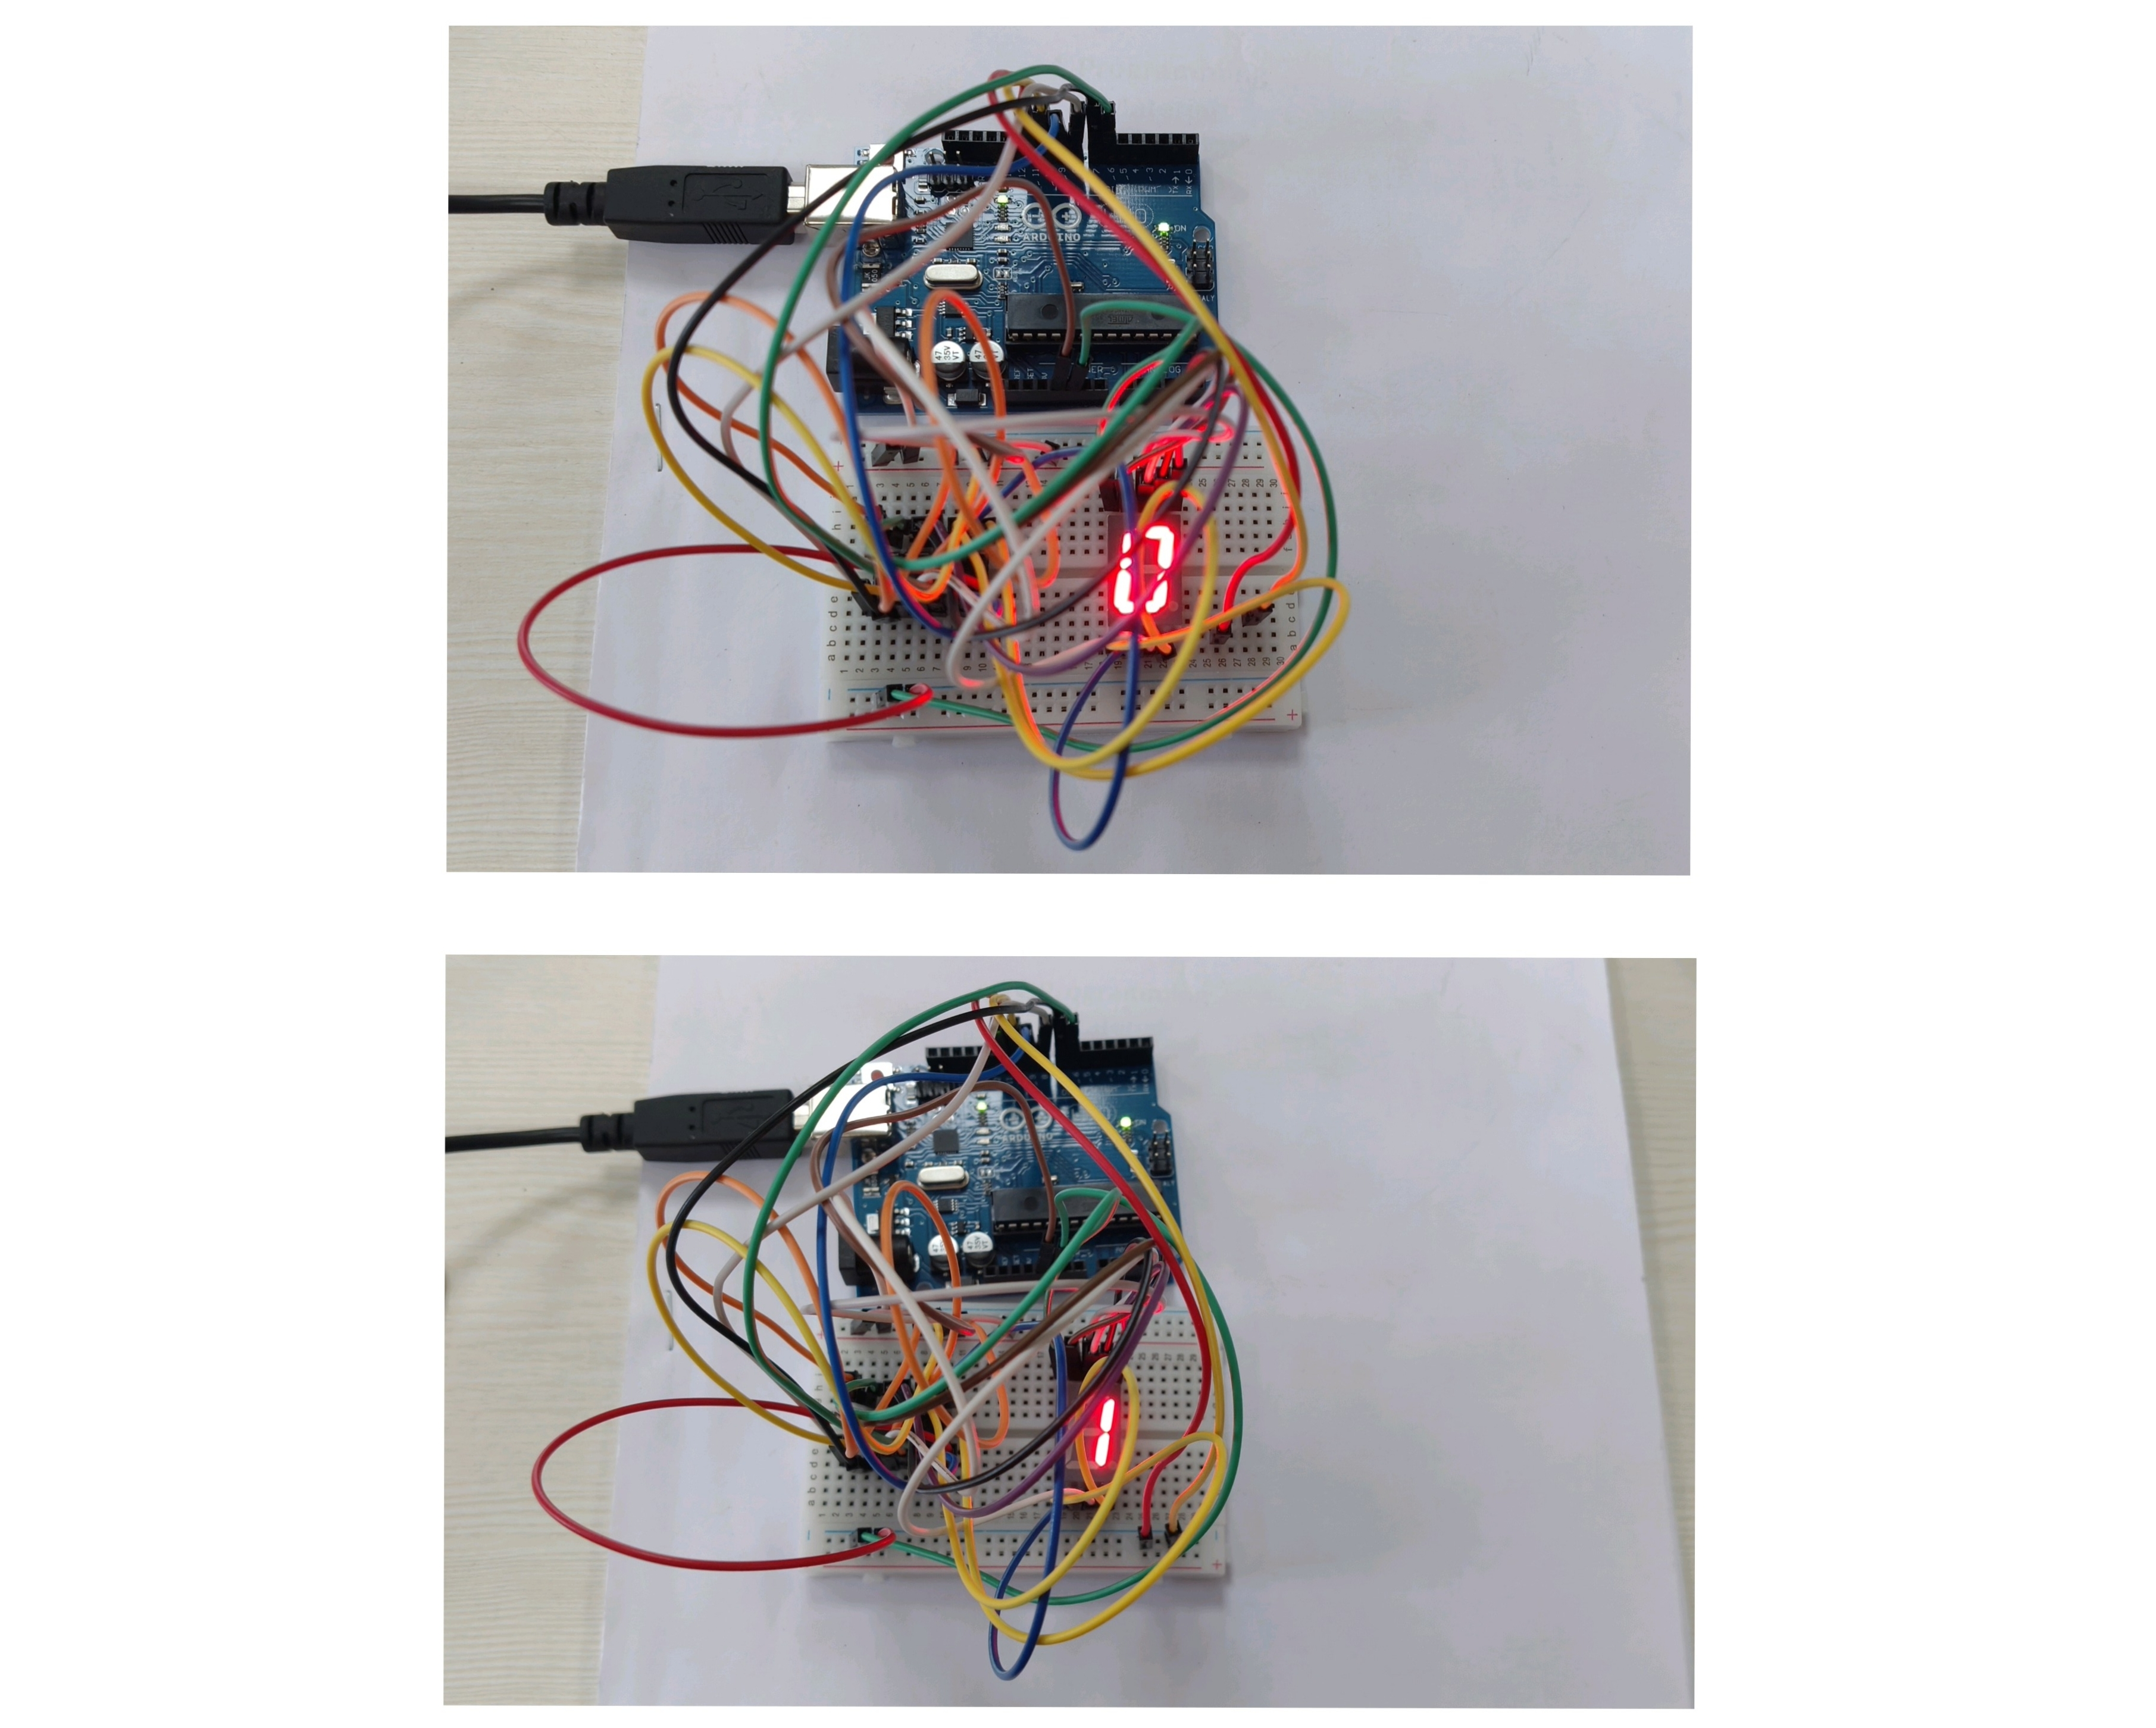
\includegraphics[width=10cm]{images/hardware.jpg}
\end{center}

\section*{Conclusion}

The Boolean expression $F = AB\overline{C}$ was verified using Arduino UNO and a seven segment display through the 7447 decoder. The experimental result matches the theoretical analysis.

\end{document}
